
\chapter{Mineração de Dados dos Alunos de Ciência da Computação da UnB} \label{chapter5}

Neste capítulo, será descrita a metodologia utilizada para a análise dos dados e obtenção dos resultados propostos, orientado pelo processo de extração do conhecimento (KDD) descrito no Capítulo \ref{chapter3}.

Na Seção \ref{5title1}, é delimitado o objeto de pesquisa, que consiste dos objetivos a serem alcançados pela mineração de dados. A Seção \ref{5subtitle1} descreve a etapa de aquisição e seleção dos dados, além ferramentas utilizadas para armazenamento e manipulação desses dados. A Seção \ref{5subtitle2} descreve a etapa de pré-processamento dos dados, listando os atributos que foram removidos da mineração. A Seção \ref{5subtitle3} descreve a etapa de transformação dos dados, que envolve a modificação e criação de atributos e tabelas, além de descrever o processo de criação dos arquivos de dados a serem minerados pelo Weka. Finalizando, a Seção \ref{5subtitle4} descreve a etapa de mineração dos dados, que envolve a análise dos dados com os algoritmos de mineração e a seleção dos algoritmos utilizados para a análise dos dados.

\section{Delimitação do Objeto de Pesquisa} \label{5title1}

Da abordagem realizada nas Seções \ref{2title53} e \ref{2title54}, é possível identificar alguns aspectos em comum nos trabalhos de \citet{dantas2014} e \citet{palmeira_santos2014}, tais como:

\begin{itemize}
	\item Os três primeiros semestres são os que registram as maiores taxas de evasão;
	\item As disciplinas de Computação Básica e Estruturas de Dados apresentam altas taxas de reprovação;
	\item As disciplinas de Matemática e Física, tais como Cálculo 1, Cálculo 2, Cálculo 3, Física 1, Física 2 e Física 3 apresentam altas taxas de reprovação;
	\item Das disciplinas ofertadas pelo CIC-UnB, Computação Básica e Estruturas de Dados estão entre as disciplinas consideradas determinantes para a continuidade ou não do curso, por serem obrigatórias dos semestres iniciais e por serem pré-requisitos para as disciplinas subsequentes;
	\item Entre as formas de evasão, a maioria ocorre por abandono de curso.
\end{itemize}

Diante dos aspectos apresentados, a análise consistirá de dados sobre os alunos do curso de Bacharelado em Ciência da Computação e seus respectivos históricos acadêmicos. 

Entre as disciplinas a serem analisadas, foram selecionadas Computação Básica, Estruturas de Dados e Programação Sistemática (CIC-UnB); Cálculo 1, Cálculo 2 e Cálculo 3 (MAT-UnB); Física 1, Física 2 e Física 3 (IF-UnB). Essas disciplinas estão distribuídas entre o primeiro e terceiro semestre do fluxo acadêmico, e são consideradas disciplinas de base para a continuidade do curso. 

Neste trabalho a mineração de dados terá a finalidade de:
\begin{itemize}
	\item Verificar as variáveis que influenciaram no processo de evasão ao longo dos semestres;
	\item Identificar regras que permitam justificar a evasão para alunos de determinado semestre;
	\item Verificar se menções ou turmas das disciplinas analisadas exercem influência sobre o processo de evasão;
	\item Identificar os principais padrões e tendências que permitam justificar a evasão dos alunos ao longo dos anos.
\end{itemize}

Uma vez definidos os objetivos a serem alcançados pela mineração de dados, a próxima etapa consiste na implementação das fases do processo extração do conhecimento (KDD), conforme explicitado na Seção \ref{3title1} do Capítulo \ref{chapter3}. As Seções \ref{5subtitle1} até \ref{5subtitle4} detalham todo o processo de mineração de dados empregado neste trabalho, com a finalidade de alcançar os objetivos propostos.


\section{Seleção dos Dados} \label{5subtitle1}

Os dados obtidos para este trabalho foram os mesmos utilizados por \citet{palmeira_santos2014}, que foram recuperados do Sistema de Informação Acadêmica de Graduação (SIGRA) e disponibilizados pelo Decanato de Planejamento e Orçamento da Universidade de Brasília (DPO). Os arquivos de dados foram entregues em formato \textit{CSV} (disponibilizados pelo DPO) e \textit{SQL} (disponibilizados por \citet{palmeira_santos2014}). Junto aos arquivos, foi entregue um dicionário de dados, a fim de facilitar a compreensão do significado dos valores numéricos para determinados atributos. 

Com o objetivo de otimizar a busca e recuperação dos registros, optou-se por trabalhar com os arquivos em formato SQL, visto que os registros já se encontravam pré-processados para serem manipulados via banco de dados. 

O banco de dados escolhido para este trabalho foi o MySQL versão 5.5.12, e como ferramenta de apoio à edição de tabelas e dados foi escolhido o HeidiSQL versão 9.2.0~\footnote{\url{http://www.heidisql.com/}}, mostrado na Figura \ref{heidisql}, devido a disponibilidade de recursos para tratamento de dados, por possuir uma interface simples e intuitiva (disponível no idioma português brasileiro), por disponibilizar um guia de ajuda para a utilização dos comandos da linguagem SQL e por ser uma ferramenta gratuita para \textit{download}. O HeidiSQL pode ser utilizado com os bancos de dados MySQL, Microsoft SQL Server e PostgreSQL.

\begin{figure}[!htb]
	\centering
	{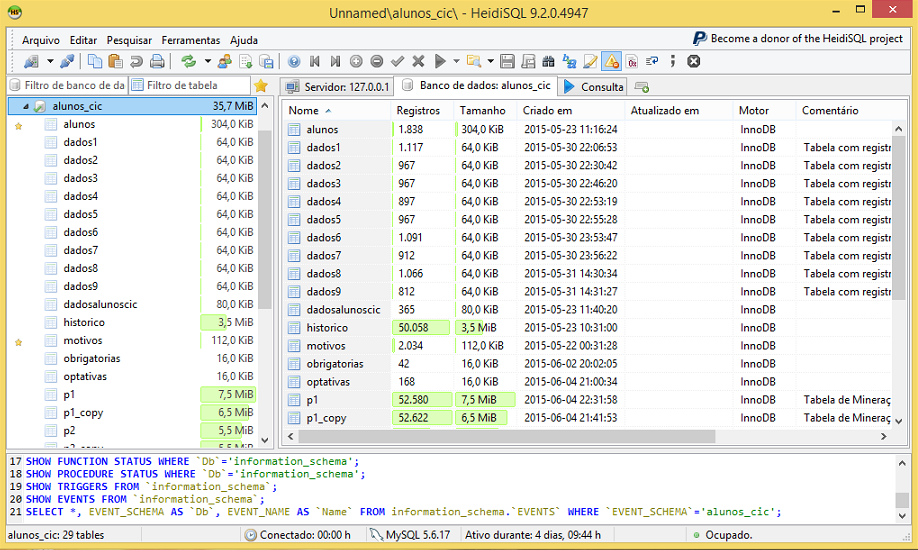
\includegraphics[width=13cm,height=8cm]{images/heidisql}}
	\caption {Interface do HeidiSQL.}
	\label{heidisql}
\end{figure}

\begin{figure}[!htb]
	\centering
	{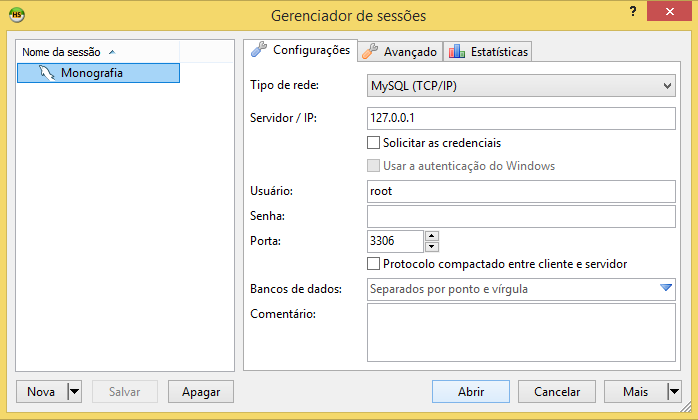
\includegraphics[width=11cm,height=7cm]{images/heidisqlinicio}}
	\caption {Tela de configuração de conexão no HeidiSQL.}
	\label{heidisqlinicio}
\end{figure}


Para manipular bases, tabelas e dados no MySQL via HeidiSQL, é necessário que o servidor do banco de dados esteja ativo. Ao executar o HeidiSQL, aparecerá a tela de configuração da conexão, conforme mostrado na Figura \ref{heidisqlinicio}. Na opção \textit{Tipo de Rede} é possível escolher o banco de dados a ser utilizado (\textit{MySQL (TCP/IP)}). O campo \textit{Servidor IP} requer o endereço IP do servidor ao qual o MySQL está vinculado (neste caso é utilizado o endereço local da máquina \textit{127.0.0.1}). Os campos \textit{Usuário, Senha} e \textit{Porta} são referentes às credencias de acesso ao banco de dados, sendo padrão o campo \textit{Usuário} como \textit{"root"}, o campo \textit{Senha} em branco (nula) e o campo \textit{Porta} como \textit{3306}.

Primeiramente, foi criada uma nova base de dados \textit{(database)}, denominada \textit{alunos\_cic}, onde foram armazenadas as tabelas criadas. Após a execução dos arquivos SQL, foram criadas quatro tabelas principais no MySQL, sendo estas:
\begin{itemize}
	\item \textit{Alunos:} Contém os dados gerais sobre os alunos ingressantes entre o primeiro semestre de 1983 e o primeiro semestre de 2014. Ao todo, foram contabilizados 2034 registros. Os atributos referentes estão descritos na Tabela \ref{5tab};
	\begin{longtable}{c|c}
		
		\caption{Atributos referentes aos alunos.} 	\label{5tab}\\
		\hline
		Atributos & Descrição\\
		\hline
			MatricAluno & Código do aluno no sistema\\
			AnoIngresso & Ano de ingresso na Universidade\\
			FormaIngresso & Forma de ingresso na Universidade\\
			SemestreIngresso & Semestre de ingresso na Universidade\\
			AnoSaida & Ano de saída da Universidade\\
			SemestreSaida & Semestre de Saída da Universidade\\
			FormaSaida & Forma de Saída da Universidade\\
			PerIngressoOpcao & Período de ingresso na opção\\
			SemestreIngressoOpcao & Semestre de ingresso na opção\\ 
			ForIngressoOpcao & Forma de ingresso na opção\\
			PerSaidaOpcao & Período de saída da opção\\
			SemestreSaidaOpcao & Semestre de saída na opção\\
			ForSaidaOpcao & Forma de saída da opção\\
			AlunoRegistrado & Se aluno está registrado ou não\\
			PeriodoCurricular & Ano do período curricular\\
			SemestrePeriodoCurricular & Semestre do período curricular\\
			AluSexo & Sexo do aluno\\
			AluNacionalidade & Nacionalidade do aluno\\
			AluDtNasc & Data de nascimento do aluno\\
			AluCotId & Sistema de ingresso do aluno\\
			AluEscola & Tipo de escola que o aluno cursou o Ensino Médio\\
		\hline
	\end{longtable}
	\item \textit{Histórico:} Contém todos os registros de histórico acadêmico dos alunos entre o ano de 2000 e 2013. Ao todo, foram contabilizados 52.900 registros. Os atributos referentes estão descritos na Tabela \ref{5tab1};
		\begin{longtable}{c|c}
			
			\caption{Atributos referentes ao histórico.} 	\label{5tab1}\\
			\hline
			Atributos & Descrição\\
			\hline
			MatricAluno & Código do aluno no sistema\\
			Ano & Ano em que a disciplina foi cursada\\
			Semestre & Semestre em que a disciplina foi cursada\\
			CodDisc & Código da Disciplina\\
			Créditos & Quantidade de créditos da disciplina\\
			Mencao & Menção obtida pelo aluno\\
			Frequencia & Quantidade de faltas, em porcentagem\\		
			\hline
		\end{longtable}
	\item \textit{Obrigatórias:} Contém informações sobre as disciplinas obrigatórias do curso. Ao todo, foram contabilizados 42 registros. Os atributos referentes estão descritos na Tabela \ref{5tab2};
	\begin{longtable}{C{4cm}|C{7cm}}
		
		\caption{Atributos referentes as disciplinas obrigatórias.} 	\label{5tab2}\\
		\hline
		Atributos & Descrição\\
		\hline
		CodDisciplina & Código da disciplina\\
		NomeDisciplina & Nome da disciplina\\
		Departamento & Departamento que oferta a disciplina\\	
		Fluxo & Semestre que a disciplina é ofertada\\	
		\hline
	\end{longtable}
	\item \textit{Optativas:} Contém informações sobre as disciplinas optativas do curso. Ao todo, foram contabilizados 168 registros. Os atributos referentes estão descritos na Tabela \ref{5tab3}.
	
		\begin{table}[!htb]
			\centering
			\caption{Atributos referentes as disciplinas optativas.} 	\label{5tab3}
			\begin{tabular}{C{3cm}|C{6cm}}
				\hline
				Atributos & Descrição\\
				\hline
				CodDisciplina & Código da disciplina\\
				NomeDisciplina & Nome da disciplina\\
				\hline
			\end{tabular}
		\end{table}
\end{itemize}

\section{Pré-processamento dos Dados} \label{5subtitle2}

Após a criação das tabelas \textit{Alunos}, \textit{Histórico}, \textit{Obrigatórias} e \textit{Optativas} no banco de dados, foi realizada uma análise a fim de identificar e remover os atributos considerados desnecessários, redundantes ou inconsistentes para o processo de mineração. Os atributos listados abaixo foram removidos, em sua maioria, por apresentarem informações redundantes ou por não serem úteis o alcance dos objetivos definidos na Seção \ref{5title1}.

Da tabela \textit{Alunos}, por apresentarem informações redundantes, foram removidos:
\begin{center}
	\textit{PerIngressoOpcao, SemestreIngressoOpcao, ForIngressoOpcao, PerSaidaOpcao, SemestreSaidaOpcao, ForSaidaOpcao, AlunoRegistrado, PeriodoCurricular, SemestrePeriodoCurricular, AluNacionalidade.}
\end{center}


Da tabela \textit{Histórico}, por não ser utilizado, foi removido:

\begin{center}
 \textit{Frequencia.}
\end{center}


Da tabela \textit{Obrigatórias}, por não serem utilizados, foram removidos:

\begin{center}
	\textit{Departamento, Fluxo.}
\end{center}


A tabela \textit{Optativas}, neste caso, foi removida completamente, visto que o foco da mineração está nas disciplinas obrigatórias dos três primeiros semestres, sendo desnecessário o seu uso.


\section{Transformação dos Dados} \label{5subtitle3}

Para facilitar a compreensão dos atributos, foram necessárias algumas modificações nas tabelas \textit{Obrigatórias} e \textit{Alunos}, além da criação de novas tabelas e atributos (colunas) no banco de dados, a serem descritas ao decorrer desta Seção.

Na tabela \textit{Obrigatórias}, a chave primária é definida pelo campo \textit{codDisciplina}, que é do tipo numérico, visto que cada disciplina possui seu próprio código. Como cada código de disciplina é composto por seis algarismos numéricos, torna-se mais difícil para o usuário identificar intuitivamente a qual disciplina o código se refere. Para facilitar a identificação das disciplinas pelo usuário, foi criado um novo atributo denominado \textit{sigla}, que é uma abreviação do nome da disciplina, composta de 3 a 5 caracteres. Para cada disciplina na tabela \textit{Obrigatorias}, foi criada uma sigla distinta. A Tabela \ref{novaObr} mostra a nova estruturação dos atributos da tabela \textit{Obrigatórias} no MySQL. A lista de disciplinas obrigatórias e suas respectivas abreviações estão disponíveis no Apêndice \ref{apendiceA}.

\begin{table}[!h]
		\caption{Nova estrutura da tabela \textit{Obrigatórias}.} 	\label{novaObr}
		\centering
	\begin{tabular}{C{4cm}|C{8cm}}
	\hline
	Coluna & Descrição\\
	\hline
	CodDisciplina & Código da disciplina\\
	NomeDisciplina & Nome da disciplina\\
	Sigla & Abreviação do nome da disciplina\\	
	\hline
		\end{tabular}
\end{table}


Na tabela \textit{Alunos}, foram realizadas algumas modificações nos atributos numéricos, que foram convertidos para valores nominais e vice-versa. Com base no dicionário de dados fornecidos junto aos arquivos de dados, os valores numéricos dos atributos \textit{FormaIngresso, FormaSaida, AluEscola} e \textit{AluCotId} foram substituídos por suas respectivas descrições. As Tabelas \ref{atualiza1}, \ref{atualiza2}, \ref{atualiza3} e \ref{atualiza4} apresentam as conversões realizadas para forma de ingresso, forma de saída, tipo de escola e tipo de cota dos alunos, baseado nos dados registrados nas tabela.

\begin{table}[!h]
	\caption{Atualização de valores para o atributo \textit{FormaIngresso}.} 	
	\label{atualiza1}
	\centering
	\begin{tabular}{C{1cm}|C{5cm}|C{8cm}}
		\hline
		Valor & Convertido para & Nomenclatura Completa\\
		\hline
		0 & Nao Informado & Não Informado\\
		1 & Vestibular &  Vestibular\\	
		2 & Trans Obrigatoria & Transferência Obrigatória\\
		3 & Trans Facultativa & Transferência Facultativa\\
		4 & Port Dipl Curso Superior & Portador de Diploma de Curso Superior\\
		5 & Acordo Cultural & Acordo Cultural-PEC\\
		6 & Convenio Intern & Convênio Internacional\\	
		7 & Matricula Cortesia & Matrícula Cortesia\\
		17 & Pas & Programa de Avaliação Seriada\\	
		20 & Convenio Andifes & Convênio Andifes\\
		24 & Pec-G Pepppfol & \\
		27 & Enem & Exame Nacional do Ensino Médio\\
		\hline
		\end{tabular}
	\end{table}
	
	
	\begin{table}[!h]
		\caption{Atualização de valores para o atributo \textit{FormaSaida}.} 	
		\label{atualiza2}
		\centering
		\begin{tabular}{C{1cm}|C{5cm}|C{8cm}}
			\hline
			Valor & Convertido para & Nomenclatura Completa\\
			\hline
			0 & Cursando & Cursando\\
			1 & Formatura & Formatura\\		
			3 & Desl Jubilamento & Desligamento por Jubilamento\\
			5 & Desl Forca de Convenio & Desligamento por Força de Convênio\\
			6 & Transferencia & Transferência\\	
			7 & Desl Voluntario & Desligamento Voluntário\\
			9 & Falecimento & Falecimento\\	
			12 & Desl Decisao Judicial & Desligamento por Decisão Judicial\\
			16 & Desl Abandono & Desligamento por Abandono\\
			17 & Desl Nao Cumpriu Condicao & Desligamento por não Cumprir Condição\\
			20 & Reprovou 3 Vezes Msm Disc Obr & Reprovou 3 Vezes a Mesma Disciplina Obrigatória\\
			21 & Novo Vestibular & Novo Vestibular\\
			\hline
		\end{tabular}
	\end{table}
	
		\begin{table}[!h]
			\caption{Atualização de valores para o atributo \textit{AluEscola}.} 	
			\label{atualiza3}
			\centering
			\begin{tabular}{C{2cm}|C{4cm}|C{5cm}}
				\hline
				Valor & Convertido para & Nomenclatura Completa\\
				\hline
				\"\#NULO!\" & Nao Informado & Não Informado\\
				0 & Nao Informado & Não Informado\\
				1 & Publica & Escola Pública\\	
				2 & Particular& Escola Particular\\	
				\hline
			\end{tabular}
		\end{table}
		
			\begin{table}[!h]
				\caption{Atualização de valores para o atributo \textit{AluCotId}.} 	
				\label{atualiza4}
				\centering
				\begin{tabular}{C{1cm}|C{6cm}|C{7cm}}
					\hline
					Valor & Convertido para & Nomenclatura Completa\\
					\hline
					0 & Universal & Universal\\
					1 & Negro & Negro\\	
					3 & Escola Publ Baixa Renda PPI & Escola Pública Baixa Renda PPI\\
					4 & Esc Publ Baixa Renda Nao PPI & Escola Pública Baixa Renda Não PPI\\
					5 & Escola Publ Alta Renda PPI & Escola Pública Alta Renda PPI\\
					6 &	Esc Publ Alta Renda Nao PPI & Escola Pública Alta Renda Não PPI\\
					\hline
				\end{tabular}
			\end{table}
	

	Após a conversão dos atributos numéricos em nominais, foi realizado um \textit{inner join}\footnote{O comando \textit{inner join} realiza a correspondência (junção) e retorna os dados de duas ou mais tabelas, desde que haja campos ou chaves correspondentes entre as tabelas.} das tabelas \textit{Alunos} e \textit{Histórico}, e os valores obtidos dessa junção foram salvos em uma nova tabela, denominada \textit{evasao\_todas}. 
	
	Além dos campos obtidos pela junção das tabelas, foram acrescentados três novos atributos na tabela \textit{evasao\_todas}, sendo estes \textit{AluSituacao}, \textit{DiscMateriaCursada} e {DiscStatusMencao}.
	
	 O atributo \textit{AluSituacao}  foi criado para definir a condição atual do aluno: \textit{"Formado"} caso o valor na coluna \textit{FormaSaida} seja "Formatura";  \textit{"Cursando"} caso o valor na coluna \textit{FormaSaida} seja "Cursando"; e \textit{"Desligado"} para os demais valores em \textit{FormaSaida}. 
	 
	 O atributo \textit{DiscMateriaCursada} foi criado com o objetivo de sintetizar os atributos \textit{Sigla} (tabela \textit{Obrigatórias}), \textit{Ano, Semestre} e \textit{Turma} (tabela \textit{Histórico}) em um único valor, por meio da função \textit{concat}~\footnote{A função \textit{concat} na linguagem SQL permite realizar a concatenação de diferentes valores em um único resultado.} no MySQL. 
	 
	 O atributo \textit{DiscStatusMencao} foi criado para identificar se o aluno foi aprovado ou reprovado em determinada disciplina com base na menção obtida. De acordo com as regras da Universidade de Brasília, ao cursar uma disciplina, o aluno poderá obter uma das seguintes menções classificadas conforme a Tabela \ref{mencoes1}.
	
		\begin{table}[!h]
			\caption{Classificação das Menções na Universidade de Brasília.} 	
			\label{mencoes1}
			\centering
			\begin{tabular}{C{2cm}|C{5cm}|C{3cm}}
				\hline
			Menção & Descrição & Nota\\
				\hline
				SR & Sem Rendimento & 0\\	
				II & Inferior & 0,1 a 2,9\\
				MI & Médio Inferior & 3,0 a 4,9\\
				MM & Médio & 5,0 a 6,9\\
				MS & Médio Superior & 7,0 a 8,9\\
				SS & Superior & 9,0 a 10,0\\
				\hline
			\end{tabular}
		\end{table}

	Caso o aluno tenha obtido menção MM, MS, SS ou CC (Crédito Concedido) para determinada disciplina, o valor do atributo \textit{DiscStatusMencao} é \textit{"Aprovado"}. Caso tenha obtido, SR, II ou MI ou tenha realizado o trancamento da disciplina, seja este parcial ou geral (TR, TJ, TM)~\footnote{TJ:Trancamento Parcial de Matrícula. Excepcional e Justificado; TR: Trancamento Parcial de Matrícula. Concessão Automática; TM: Trancamento Geral de Matrícula. Automático e justificado.} o valor do atributo \textit{DiscStatusMencao} é \textit{"Reprovado"}.
	
	Por último, os valores para o atributo \textit{DtNasc} também foram modificados, convertidos de nominais para numéricos. Da data de nascimento dos alunos, foram desprezados os valores do dia e do mês, considerando-se somente o ano.
	
	Após a criação e edição dos atributos na tabela \textit{evasao\_todas}, foi realizada uma cópia da mesma, incluindo os valores dos dados, e salva no banco de dados como \textit{evasao\_obrigatorias}. Nessa nova tabela, foram removidos os dados referentes às disciplinas optativas, visto que estes dados não serão objeto de análise para este trabalho.    
	
	\subsection{Organização dos Dados por Departamento e Disciplinas} \label{5subsubtitle1}
	
	Além das tabelas \textit{evasao\_todas} e \textit{evasao\_obrigatorias}, foram criadas outras três tabelas: \textit{evasao\_cic}, \textit{evasao\_mat} e \textit{evasao\_fis}, contendo dados sobre as disciplinas organizadas por departamento. A tabela \textit{evasao\_cic} contém dados de Computação Básica, Estruturas de Dados e Programação Sistemática; a tabela \textit{evasao\_mat} contém dados de Cálculo 1, Cálculo 2 e Cálculo 3; e  a tabela \textit{evasao\_fis} contém dados de Física 1, Física 2 e Física 3, que foram as disciplinas definidas na Seção \ref{5title1}.  
	
	Para realizar a recuperação e armazenamento dos dados, foi desenvolvido uma aplicação em Java (vide Apêndice \ref{apendiceB}) e executada na IDE~\footnote{IDE - \textit{Integrated Development Environment}, ou \textit{Ambiente Integrado de Desenvolvimento.}} Eclipse, capaz de contar a quantidade de vezes que determinada disciplina foi cursada, recuperar a primeira e última menção obtida pelo aluno, e recuperar a primeira e última turma na qual a disciplina foi cursada da tabela \textit{historico}. Tomando por base a disciplina pré-requisito do primeiro semestre de cada departamento, o método captura as informações para as disciplinas subsequentes, conforme mostrado na Figura \ref{metodoJava}. Por exemplo, a partir dos alunos que cursaram Computação Básica, foram verificados os registros para os alunos que cursaram Estruturas de dados; e a partir dos alunos que cursaram Estruturas de Dados, foram verificados os registros para os alunos que cursaram Programação Sistemática. 
	
	
	
	\begin{figure}[!htb]
		\centering
		{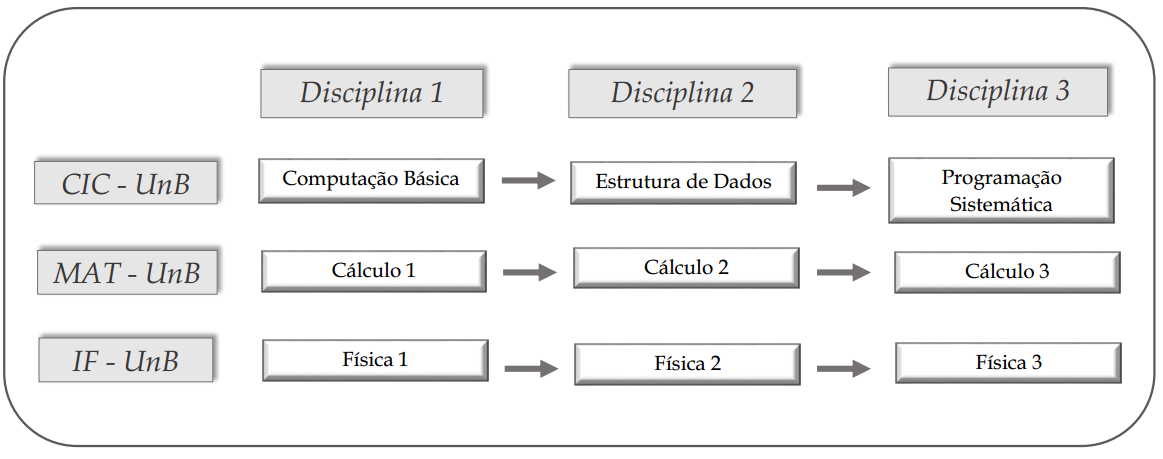
\includegraphics[width=10cm, height=4cm]{images/analiseJava}}
		\caption {Fluxo de Análise das Disciplinas pela aplicação Java. A partir da disciplina pré-requisito do primeiro semestre de cada departamento, foi verificado o histórico do aluno para as disciplinas subsequentes.}
		\label{metodoJava}
	\end{figure}
	
		\begin{figure}[!htb]
			\centering
			{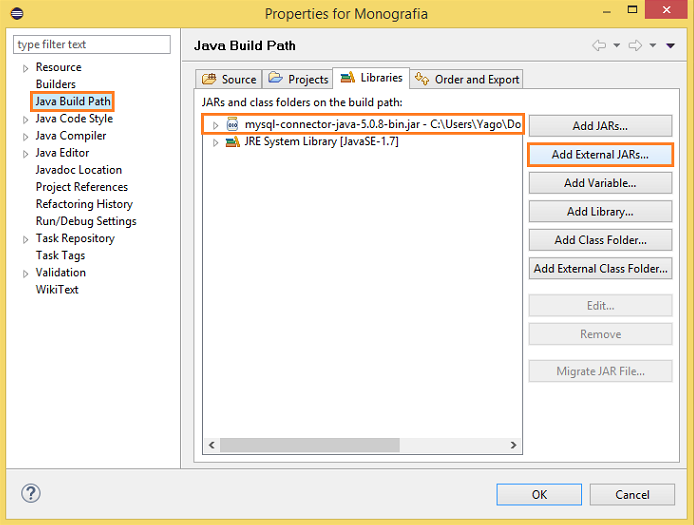
\includegraphics[width=12cm, height=7cm]{images/driverEclipse}}
			\caption {Adicionando o \textit{driver} JBDC ao Projeto no Eclipse.}
			\label{driverJBDC}
		\end{figure}
	
	Para realizar a integração entre o MySQL e a IDE Eclipse, foi necessário baixar o \textit{driver} JBDC~\footnote{O driver pode ser obtido em \url{http://dev.mysql.com/downloads/connector/j/5.1.html}.} do MySQL. Após a obtenção do \textit{driver}, o mesmo foi adicionado à biblioteca do projeto que contém o método utilizado, clicando com o botão direito sobre a pasta do projeto no Eclipse e em seguida selecionando a opção \textit{Properties}. Na nova janela aberta, foi selecionada a opção \textit{Java Build Path} e em seguida a opção \textit{Add External JARs}, conforme mostrado na Figura \ref{driverJBDC}. O \textit{driver} consiste em um arquivo em formato JAR \textit{(Java Archive)}. Com o \textit{driver} JBDC adicionado ao projeto, tornou-se possível realizar consultas SQL e atualizações de tabelas via código Java. 
	
	
	As estruturas de \textit{evasao\_cic, evasao\_mat} e \textit{evasao\_fis} são representadas pelas Tabelas \ref{evasao-cic}, \ref{evasao-mat} e \ref{evasao-fis}. Para cada aluno registrado, foram recuperados a quantidade de vezes que a disciplina foi cursada, a primeira e última nota obtida para a disciplina e a primeira e última turma na qual a disciplina foi cursada, além do \textit{status} da última menção obtida pelo aluno \textit{(aprovado/reprovado)}.

	
		\begin{longtable}{C{4cm}|C{12cm}}
			\caption{Estrutura da Tabela \textit{evasao\_cic}.} 	\label{evasao-cic}\\
				\hline
				Coluna & Descrição\\
				\hline
				Matricula & Matrícula do aluno no sistema\\
				QtdeCB & Quantidade de vezes que Computação Básica foi cursada\\
				PrimeiraNotaCB & Primeira nota obtida em Computação Básica\\
				PrimeiraTurmaCB & Primeira turma cursada de Computação Básica\\
				UltimaNotaCB & Última nota obtida em Computação Básica\\
				UltimaTurmaCB & Última turma cursada de Computação Básica\\
				StatusMencaoCB & Aprovação ou Reprovação do aluno ao cursar Computação Básica pela última vez\\
				QtdeED & Quantidade de vezes que Estruturas de Dados foi cursada\\
				PrimeiraNotaED & Primeira nota obtida em Estruturas de Dados\\
				PrimeiraTurmaED & Primeira turma cursada de Estruturas de Dados\\
				UltimaNotaED & Última nota obtida em Estruturas de Dados\\
				UltimaTurmaED & Última turma cursada de Estruturas de Dados\\
				StatusMencaoED & Aprovação ou Reprovação do aluno ao cursar Estruturas de Dados pela última vez\\
				QtdePS & Quantidade de vezes que Programação Sistemática foi cursada\\
				PrimeiraNotaPS & Primeira nota obtida em Programação Sistemática\\
				PrimeiraTurmaPS & Primeira turma cursada de Programação Sistemática\\
				UltimaNotaPS & Última nota obtida em Programação Sistemática\\
				UltimaTurmaPS & Última turma turma cursada de Programação 
				Sistemática\\
				StatusMencaoPS & Aprovação ou Reprovação do aluno ao cursar Programação Sistemática pela última vez\\
				\hline
		\end{longtable}
	
		\begin{longtable}{C{4cm}|C{12cm}}
			\caption{Estrutura da Tabela \textit{evasao\_mat}.} \label{evasao-mat}\\
			\hline
			Coluna & Descrição\\
			\hline
			Matricula & Matrícula do aluno no sistema\\
			QtdeC1 & Quantidade de vezes que Cálculo 1 foi cursada\\
			PrimeiraNotaC1 & Primeira nota obtida em Cálculo 1\\
			PrimeiraTurmaC1 & Primeira turma cursada de Cálculo 1\\
			UltimaNotaC1 & Última nota obtida em Cálculo 1\\
			UltimaTurmaC1 & Última turma cursada de Cálculo 1\\
			StatusMencaoC1 & Aprovação ou Reprovação do aluno ao cursar Cálculo 1 pela última vez\\
			QtdeC2 & Quantidade de vezes que Cálculo 2 foi cursada\\
			PrimeiraNotaC2 & Primeira nota obtida em Cálculo 2\\
			PrimeiraTurmaC2 & Primeira turma cursada de Cálculo 2\\
			UltimaNotaC2 & Última nota obtida em Cálculo 2\\
			UltimaTurmaC2 & Última turma cursada de Cálculo 2\\
			StatusMencaoC2 & Aprovação ou Reprovação do aluno ao cursar Cálculo 2 pela última vez\\
			QtdeC3 & Quantidade de vezes que Cálculo 3 foi cursada\\
			PrimeiraNotaC3 & Primeira nota obtida em Cálculo 3\\
			PrimeiraTurmaC3 & Primeira turma cursada de Cálculo 3\\
			UltimaNotaC3 & Última nota obtida em Cálculo 3\\
			UltimaTurmaC3 & Última turma turma cursada de Cálculo 3\\
			StatusMencaoC3 & Aprovação ou Reprovação do aluno ao cursar Cálculo 3 pela última vez\\
			\hline
		\end{longtable}
		
				\begin{longtable}{C{4cm}|C{12cm}}
					\caption{Estrutura da Tabela \textit{evasao\_fis}.} \label{evasao-fis}\\
						\hline
						Coluna & Descrição\\
						\hline
						Matricula & Matrícula do aluno no sistema\\
						QtdeF1 & Quantidade de vezes que Física 1 foi cursada\\
						PrimeiraNotaF1 & Primeira nota obtida em Física 1\\
						PrimeiraTurmaF1 & Primeira turma cursada de Física 1\\
						UltimaNotaF1 & Última nota obtida em Física 1\\
						UltimaTurmaF1 & Última turma cursada de Física 1\\
						StatusMencaoF1 & Aprovação ou Reprovação do aluno ao cursar Física 1 pela última vez\\
						QtdeF2 & Quantidade de vezes que Física cursada\\
						PrimeiraNotaF2 & Primeira nota obtida em Física 2\\
						PrimeiraTurmaF2 & Primeira turma cursada de Física 2\\
						UltimaNotaF2 & Última nota obtida em Física 2\\
						UltimaTurmaF2 & Última turma cursada de Física 2\\
						StatusMencaoF2 & Aprovação ou Reprovação do aluno ao cursar Física 2 pela última vez\\
						QtdeF3 & Quantidade de vezes que Física 3 foi cursada\\
						PrimeiraNotaF3 & Primeira nota obtida em Física 3\\
						PrimeiraTurmaF3 & Primeira turma cursada de Física 3\\
						UltimaNotaF3 & Última nota obtida em Física 3\\
						UltimaTurmaF3 & Última turma turma cursada de Física 3\\
						StatusMencaoF3 & Aprovação ou Reprovação do aluno ao cursar Física 3 pela última vez\\
						\hline
				\end{longtable}

\subsection{Geração dos Arquivos em Formato ARFF} \label{5subsubtitle2}

Após a criação das tabelas e organização dos dados, foi necessária a conversão dos registros armazenados no MySQL para o formato ARFF \textit{(Attribute-Relation File Format,} ou \textit{Arquivo em Formato Atributo-Relação}), que é o formato padrão utilizado pelo Weka para realização da mineração de dados \citep{witten2005}. Segundo \citet{witten2005}, o arquivo em formato ARFF apenas fornece o conjunto de dados, não especificando quais atributos devem ser utilizados para classificação. O mesmo arquivo ARFF pode ser utilizado para analisar a forma como cada atributo pode ser classificado a partir de outros atributos, encontrar regras de associação ou identificar agrupamentos \textit{(clusters)}.

 Uma das possibilidades de criar arquivos de dados em formato ARFF é através do próprio Weka, por meio de integração entre o \textit{software} e o MySQL. Da mesma forma que o Eclipse, o Weka requer o \textit{driver} JBDC do MySQL para possibilitar a conexão ao banco de dados.

\subsubsection{Integrando o Weka ao MySQL} \label{sub51}

Para configurar o Weka no sistema operacional \textit{Windows}, torna-se necessária a realização dos seguintes procedimentos:
\begin{itemize}
	\item Salve o \textit{driver} do MySQL na pasta do projeto Weka; 
	\item Na pasta do Weka, clique com o botão direito do mouse sobre o arquivo \textit{weka.jar (Executable Jar File)}, e em seguida, escolha a opção \textit{Abrir com o WinRAR}. Caso não utilize o \textit{WinRAR}, pode-se optar por outro descompactador de arquivos e pastas;
	
	 \begin{figure}[!h]
	 	\centering
	 	{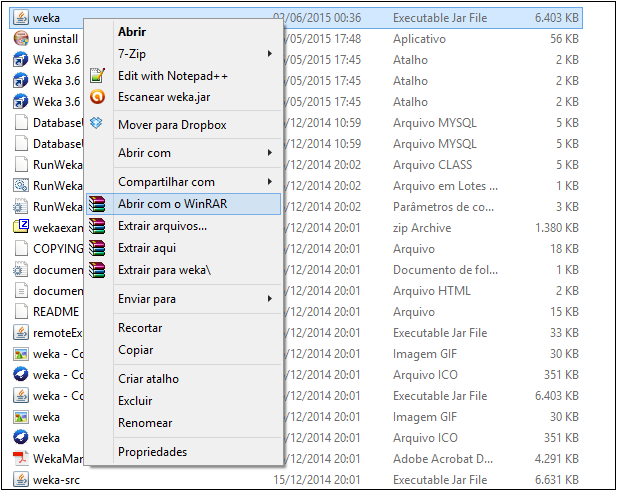
\includegraphics[width=11cm, height=8cm]{images/winrar}}
	 	\caption {Acesso ao arquivo \textit{weka.jar} para configurar a integração entre o Weka e o MySQL.}
	 	\label{winrar}
	 \end{figure}
	 
	 \item Ao abrir o arquivo \textit{weka.jar} com o \textit{WinRAR}, aparecerá um diretório contendo três pastas, sendo estas \textit{java\_cup, META-INF} e \textit{Weka}. Selecione a pasta \textit{Weka}, e em seguida a pasta \textit{experiment}. Na pasta \textit{experiment}, abra o arquivo \textit{DataBaseUtilsmysql.props} com o auxílio de algum editor de textos (Notepad++, Bloco de Notas, Wordpad...), conforme mostrado na Figura \ref{winrar2};
	 
	   \begin{figure}[!h]
	   	\centering
	   	{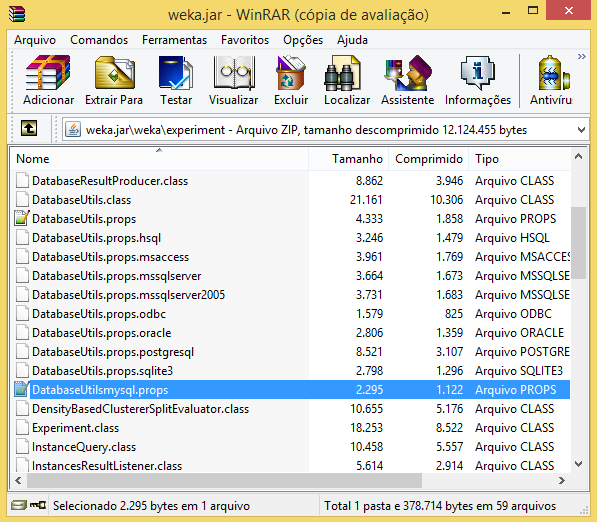
\includegraphics[width=11cm, height=8cm]{images/winrar2}}
	   	\caption {Diretório de acesso ao arquivo \textit{DataBaseUtilsmysql.props} }
	   	\label{winrar2}
	   \end{figure}
	   
	   \item Após abrir o arquivo com o editor de textos, informe o \textit{driver} utilizado do MySQL no campo \textit{jdbcDriver}, e a URL de acesso ao banco de dados no campo \textit{jdbcURL}, conforme mostrado na Figura \ref{winrar3}. Para este trabalho, o \textit{driver} do MySQL utilizado foi o \textit{com.mysql.jdbc.Driver};
	   
	    \begin{figure}[!h]
	    	\centering
	    	{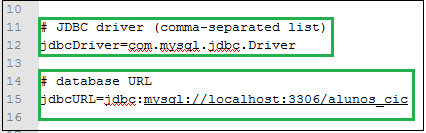
\includegraphics[width=9cm, height=3cm]{images/winrar3}}
	    	\caption {Declaração do \textit{driver} utilizado do MySQL e da URL de acesso ao banco de dados no arquivo \textit{DataBaseUtilsmysql.props.}}
	    	\label{winrar3}
	    \end{figure}
	    
	   \item Na seção \textit{specific data types} do arquivo \textit{DataBaseUtilsmysql.props}, são declarados os tipos de dados a serem utilizados. Para este trabalho, foram utilizados dados do tipo \textit{INT, INTEGER, FLOAT} e \textit{LONG} para dados do tipo númerico, \textit{VARCHAR} e \textit{TEXT} para dados do tipo texto, e \textit{BIT} para dados do tipo binário, conforme mostrado na Figura \ref{winrar4};
	   
	        \begin{figure}[!h]
	        	\centering
	        	{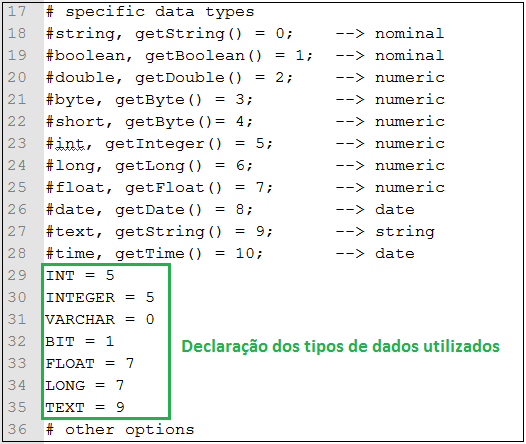
\includegraphics[width=10cm, height=7cm]{images/winrar4}}
	        	\caption {Declaração do \textit{driver} utilizado do MySQL e da URL de acesso ao banco de dados no arquivo \textit{DataBaseUtilsmysql.props.}}
	        	\label{winrar4}
	        \end{figure}
	   
	   \item Salve o arquivo após as modificações realizadas. Em seguida, renomeie-o para \textit{DataBaseUtils.props}, dentro da própria pasta;
	   
	   \item Realizada a alteração no arquivo, execute o Weka via \textit{Prompt de Comando}. Para executar o Weka junto ao MySQL, informe o seguinte comando:
	   \newline
	   \begin{center}
	   	\textit{java -cp <caminho do \textit{driver} MySQL na pasta Weka>; <caminho do diretório do arquivo \textit{weka.jar}> weka.gui.GUIChooser}
	   \end{center}
	   
	   O comando \textit{-cp} é utilizado pelo Java para indicar quais diretórios devem ser pesquisados para encontrar as bibliotecas necessárias para que o programa seja executado \citep{tutorial_weka}. Os diretórios devem ser separados por ponto e vírgula. Um exemplo é mostrado na Figura \ref{winrar5}. Ao executar o comando, o Weka iniciará automaticamente;
	   
	   \begin{figure}[!h]
	   	\centering
	   	{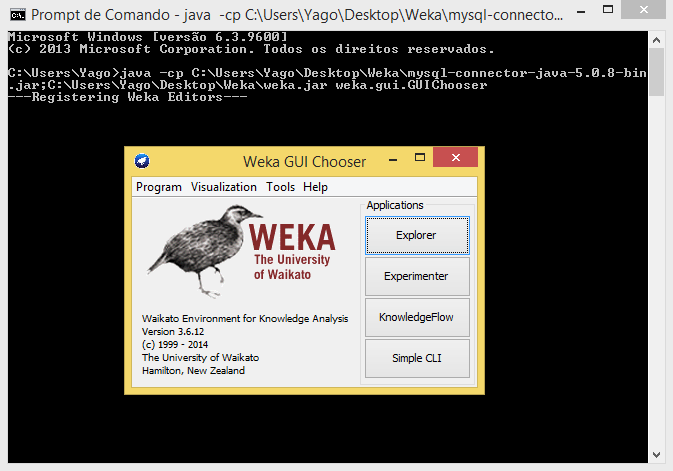
\includegraphics[width=13cm, height=10cm]{images/winrar5}}
	   	\caption {Iniciando o Weka e o MySQL via \textit{Prompt de Comando} do \textit{Windows}.}
	   	\label{winrar5}
	   \end{figure}
	   
	   \item Realizados os procedimentos de configuração, o Weka poderá ser iniciado normalmente pelo atalho \textit{Weka 3.6}.
\end{itemize}
 
\subsubsection{Recuperação dos Dados pelo Weka e Transformação para o Formato ARFF}

Após a configuração do Weka para integrar-se ao MySQL descrita na Seção \ref{sub51}, os arquivos em formato ARFF foram gerados a partir dos seguintes procedimentos:

\begin{itemize}
	\item Abrir o Weka em modo \textit{Explorer};
	\item Na guia de menus, escolher a opção \textit{Open DB...};
	\item No campo \textit{URL}, informar a URL de acesso a base de dados, e em seguida, escolher a opção \textit{User...};
	\item Ao abrir a janela \textit{Database Connection Parameters}, informar a URL de acesso ao banco de dados e as permissões de acesso, conforme mostrado na Figura \ref{weka5};
	
	 \begin{figure}[!h]
	 	\centering
	 	{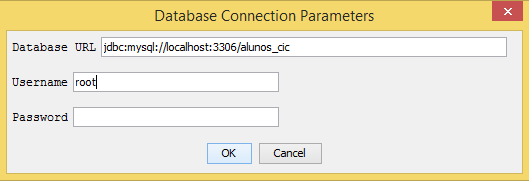
\includegraphics[width=8cm, height=2cm]{images/weka5}}
	 	\caption {Permissões de acesso ao banco de dados no Weka}
	 	\label{weka5}
	 \end{figure}
	
	\item  Em seguida, escolher a opção \textit{Connect}. Caso a conexão seja estabelecida, aparecerá a mensagem \textit{connecting to: <base de dados> =true};
	\item Informe a \textit{query} a ser utilizada e clique na opção \textit{Execute}. Após o retorno dos dados da consulta, clique em \textit{OK}. Os dados serão mostrados no Weka conforme apresentação da Figura \ref{weka6};
	
		 \begin{figure}[!h]
		 	\centering
		 	{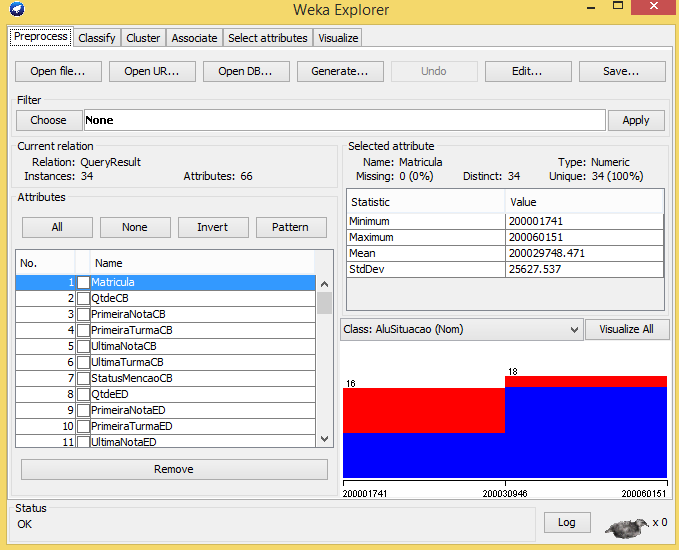
\includegraphics[width=10cm, height=9cm]{images/weka6}}
		 	\caption {Dados recuperados do SQL mostrados no Weka.}
		 	\label{weka6}
		 \end{figure}
	
	\item Agora, basta escolher a opção \textit{Save...} que o arquivo será salvo em formato ARFF.
\end{itemize}

Os procedimentos descritos nesta Seção foram realizados para os dados gerais dos alunos (todos os alunos que possuem histórico no departamento entre 2000 e 2013), e para os dados gerais dos alunos separados por semestre entre 2000 e 2013. Ao todo, foram criados 29 arquivos em formato ARFF. As \textit{querys} utilizadas para criação dos arquivos estão disponíveis no Apêndice \ref{apendiceC}.

Cada arquivo ARFF é composto dos seguintes atributos, conforme mostrado na Tabela \ref{arff}.

	\begin{longtable}{C{4cm}|C{12cm}}
		\caption{Atributos presentes no arquivo ARFF.} \label{arff}\\
		\hline
		Coluna & Descrição\\
		\hline
		Matricula & Matrícula do aluno no sistema\\
		QtdeCB & Quantidade de vezes que Computação Básica foi cursada\\
		PrimeiraNotaCB & Primeira nota obtida em Computação Básica\\
		PrimeiraTurmaCB & Primeira turma cursada de Computação Básica\\
		UltimaNotaCB & Última nota obtida em Computação Básica\\
		UltimaTurmaCB & Última turma cursada de Computação Básica\\
		StatusMencaoCB & Aprovação ou Reprovação do aluno ao cursar Computação Básica pela última vez\\
		QtdeED & Quantidade de vezes que Estruturas de Dados foi cursada\\
		PrimeiraNotaED & Primeira nota obtida em Estruturas de Dados\\
		PrimeiraTurmaED & Primeira turma cursada de Estruturas de Dados\\
		UltimaNotaED & Última nota obtida em Estruturas de Dados\\
		UltimaTurmaED & Última turma cursada de Estruturas de Dados\\
		StatusMencaoED & Aprovação ou Reprovação do aluno ao cursar Estruturas de Dados pela última vez\\
		QtdePS & Quantidade de vezes que Programação Sistemática foi cursada\\
		PrimeiraNotaPS & Primeira nota obtida em Programação Sistemática\\
		PrimeiraTurmaPS & Primeira turma cursada de Programação Sistemática\\
		UltimaNotaPS & Última nota obtida em Programação Sistemática\\
		UltimaTurmaPS & Última turma turma cursada de Programação 
		Sistemática\\
		StatusMencaoPS & Aprovação ou Reprovação do aluno ao cursar Programação Sistemática pela última vez\\
		QtdeC1 & Quantidade de vezes que Cálculo 1 foi cursada\\
		PrimeiraNotaC1 & Primeira nota obtida em Cálculo 1\\
		PrimeiraTurmaC1 & Primeira turma cursada de Cálculo 1\\
		UltimaNotaC1 & Última nota obtida em Cálculo 1\\
		UltimaTurmaC1 & Última turma cursada de Cálculo 1\\
		StatusMencaoC1 & Aprovação ou Reprovação do aluno ao cursar Cálculo 1 pela última vez\\
		QtdeC2 & Quantidade de vezes que Cálculo 2 foi cursada\\
		PrimeiraNotaC2 & Primeira nota obtida em Cálculo 2\\
		PrimeiraTurmaC2 & Primeira turma cursada de Cálculo 2\\
		UltimaNotaC2 & Última nota obtida em Cálculo 2\\
		UltimaTurmaC2 & Última turma cursada de Cálculo 2\\
		StatusMencaoC2 & Aprovação ou Reprovação do aluno ao cursar Cálculo 2 pela última vez\\
		QtdeC3 & Quantidade de vezes que Cálculo 3 foi cursada\\
		PrimeiraNotaC3 & Primeira nota obtida em Cálculo 3\\
		PrimeiraTurmaC3 & Primeira turma cursada de Cálculo 3\\
		UltimaNotaC3 & Última nota obtida em Cálculo 3\\
		UltimaTurmaC3 & Última turma turma cursada de Cálculo 3\\
		StatusMencaoC3 & Aprovação ou Reprovação do aluno ao cursar Cálculo 3 pela última vez\\
		QtdeF1 & Quantidade de vezes que Física 1 foi cursada\\
		PrimeiraNotaF1 & Primeira nota obtida em Física 1\\
		PrimeiraTurmaF1 & Primeira turma cursada de Física 1\\
		UltimaNotaF1 & Última nota obtida em Física 1\\
		UltimaTurmaF1 & Última turma cursada de Física 1\\
		StatusMencaoF1 & Aprovação ou Reprovação do aluno ao cursar Física 1 pela última vez\\
		QtdeF2 & Quantidade de vezes que Física cursada\\
		PrimeiraNotaF2 & Primeira nota obtida em Física 2\\
		PrimeiraTurmaF2 & Primeira turma cursada de Física 2\\
		UltimaNotaF2 & Última nota obtida em Física 2\\
		UltimaTurmaF2 & Última turma cursada de Física 2\\
		StatusMencaoF2 & Aprovação ou Reprovação do aluno ao cursar Física 2 pela última vez\\
		QtdeF3 & Quantidade de vezes que Física 3 foi cursada\\
		PrimeiraNotaF3 & Primeira nota obtida em Física 3\\
		PrimeiraTurmaF3 & Primeira turma cursada de Física 3\\
		UltimaNotaF3 & Última nota obtida em Física 3\\
		UltimaTurmaF3 & Última turma turma cursada de Física 3\\
		StatusMencaoF3 & Aprovação ou Reprovação do aluno ao cursar Física 3 pela última vez\\
		AluSexo & Sexo do aluno\\
		AluDtNasc & Data de nascimento do aluno\\
		AluEscola & Tipo de escola que o aluno cursou o Ensino Médio\\
		AluCotTipo & Sistema de ingresso do aluno\\
		AluAnoIngresso & Ano de ingresso na Universidade\\
		AluSemestreIngresso & Semestre de ingresso na Universidade\\
		AluAnoSaida & Ano de saída da Universidade\\
		AluSemestreSaida & Semestre de Saída da Universidade\\
		SemestreCursoSaida & Quantidade de semestres que o aluno cursou até o momento do desligamento\\
		AluSaidaMotivo & Motivo pelo qual o aluno foi desligado\\
		AluSituacao & Situação do aluno na base de dados (cursando, formado ou desligado)\\
		\hline
	\end{longtable}
				

	
\section{Mineração de Dados} \label{5subtitle4}

Após a etapa de transformação dos dados e geração dos arquivos em formato ARFF, os dados foram minerados no Weka utilizando os algoritmos de árvore de decisão \textit{(trees)}, algoritmos de regras \textit{(rules)} e os algoritmos meta-heurísticos \textit{(meta)}. Para este trabalho, optou-se por utilizar algoritmos destas tipologias pelo fato de gerarem padrões de classificação de fácil entendimento e interpretação, o que permite descobrir padrões e semelhanças entre as regras construídas pelos algoritmos.

Utilizando o \textit{software} Weka em modo \textit{Explorer}, os arquivos foram pré-processados, onde foram retirados os atributos considerados desnecessários para o processo de mineração. Para os arquivos gerados entre o ano de 2000 a 2008, foram removidos os atributos \textit{MatricAluno} e \textit{AluSaidaMotivo}, visto que a maioria dos algoritmos utilizavam apenas a segunda informação para classificar a condição do aluno. Para os arquivos gerados a partir de 2008, foram removidos os atributos \textit{MatricAluno, AluSaidaMotivo, AluAnoSaida, AluSemestreSaida} e \textit{SemestreCursoSaida}, visto que a partir de 2008 grande parte dos alunos constavam como cursando, sendo estes atributos inválidos para a mineração. Para o arquivo com todos os dados entre 2000 e 2013, foram considerados apenas as primeiras notas de cada disciplina, o sexo (masculino ou feminino) e a situação (cursando, formado ou desligado) do aluno.

Após a remoção dos atributos, foram aplicados os algoritmos de mineração sobre os dados. Pela opção \textit{Classify}, na barra de menu do Weka, é possível escolher os algoritmos a serem utilizados para a mineração, ao acessar a opção \textit{Chooser}, conforme mostrado nas Figuras \ref{classificador} e \ref{classificador2}.

   \begin{figure}[!h]
   	\centering
   	{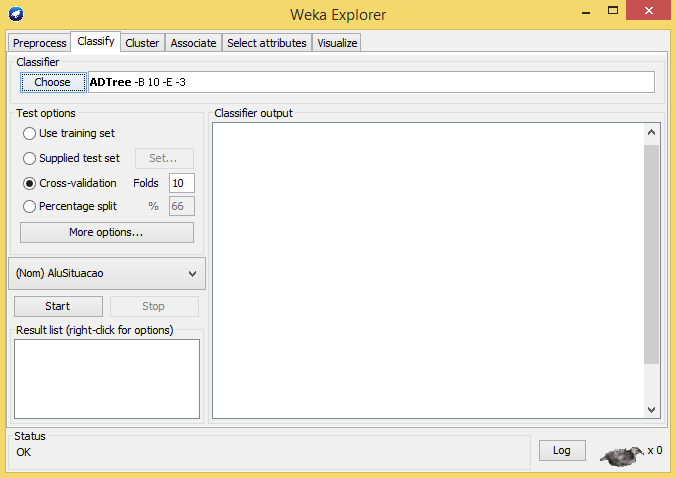
\includegraphics[width=11cm, height=8cm]{images/classificador}}
   	\caption {Tela de acesso aos algoritmos no Weka}
   	\label{classificador}
   \end{figure}
   
   \begin{figure}[!h]
   	\centering
   	{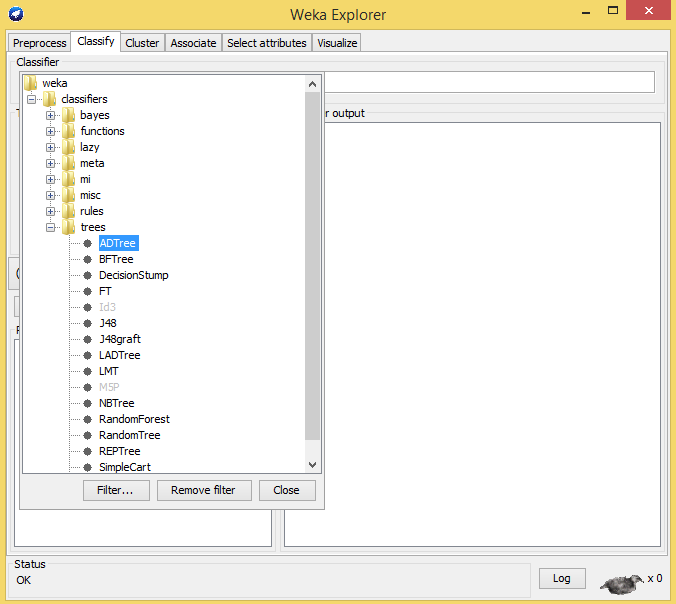
\includegraphics[width=10cm, height=8cm]{images/classificador2}}
   	\caption {Opções de algoritmos disponíveis no Weka}
   	\label{classificador2}
   \end{figure}

Entre as opções de teste, foi utilizada \textit{Cross-validation}, com o valor \textit{Folds} igual a 10. De acordo com \citet{witten2005}, o \textit{cross-validation} (ou \textit{validação cruzada}) realiza o processo de decisão sobre um número fixo de partições dos dados, onde dado um número de \textit{N} partições, são utilizadas \textit{N-1} partições para treinamento e o restante é utilizado para teste. A forma padrão de predizer uma técnica de aprendizagem dada uma amostra única e fixa de dados é utilizar a estratificação da validação cruzada 10 vezes, onde os dados são divididos aleatoriamente em 10 partes. Por padrão, o valor 10 é utilizado, onde 9 partições são utilizadas para treinamento e 1 para teste, porém o número de partições pode ser variável. As 10 estimativas de erros geradas pelas partições são calculadas para produzir uma estimativa de erro global.

O atributo escolhido para classificação foi o \textit{AluSituacao}, a partir do qual os algoritmos construíram regras para identificar a situação do aluno como \textit{cursando, formado} ou \textit{desligado}. Para cada arquivo ARFF analisado, foram identificados os algoritmos que geraram as melhores regras e conseguiram identificar o maior número de instâncias corretamente. A Figura \ref{weka5_mineracao} mostra os algoritmos previamente selecionados que apresentaram os melhores resultados para os dados de alunos ingressos no segundo semestre de 2005.

\begin{figure}[!h]
	\centering
	{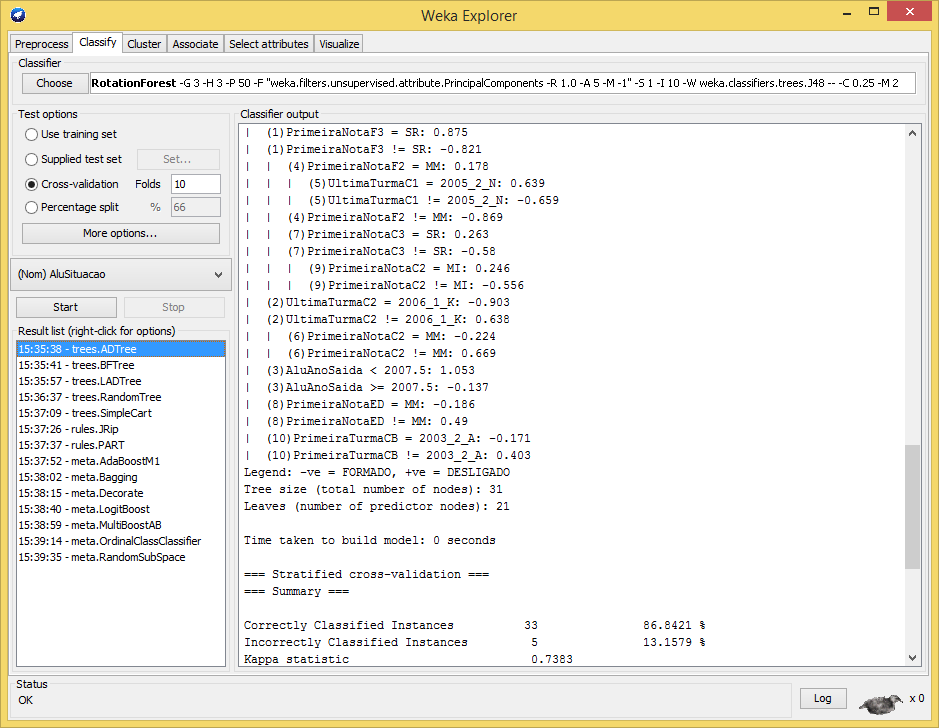
\includegraphics[width=11cm, height=10cm]{images/weka_mineracao}}
	\caption {Algoritmos selecionados para a análise dos dados de alunos ingressos no segundo semestre de 2005}
	\label{weka5_mineracao}
\end{figure}



